\chapter{Credit Default Swaps}\label{credit_default_swaps}

\section{Credit curves}\label{credit-curves}

Just like a discount curve is a way of representing the underlying
interest rates implicit in the market quotes of a collection of
real-world interest rate products, \textbf{credit curves} are a way of
representing survival probabilities implied by credit default swaps.

In fact \textbf{Credit default swaps} (\textbf{CDS}) are instruments whose value
depends on the likelihood that a given company (the curve's
\textbf{issuer}) will suffer a credit event over a given period.

A \textbf{credit event} can be a default, the failure to make payments,
the issuer entering into bankruptcy proceedings, or the occurrence of
other legal events. The exact definition of what constitutes a credit
event depends on a series of factors and is usually defined in some kind
of ISDA (International Swaps and Derivatives Association) master
agreement.

In any case, we will generically call a credit event a \emph{default},
and talk about \textbf{non-default probabilities} (\textbf{NDP}, or
survival probability), i.e.~the probability that the issuer will
not suffer a credit event \textbf{before} a given value date(i.e. non-default probability is a cumulative probability).

NDPs are the equivalent for credit curves of discount factors for
discount curves. Just like discount curves, credit curves are built by
specifying a observation date, a sequence of pillar dates and a
sequence of NDPs. 

Finally the \textbf{hazard rate} is the credit curve
equivalent of the short rate or overnight rate for discount curves. It
represents the instantaneous probability of the issuer defaulting
conditioned on it not having defaulted until that moment (in
practice we'll calculate it numerically, and therefore it'll be the, \emph{annualized}, conditional probability of the issuer defaulting between
the value date and the day after).

Table~\ref{tab:discount_vs_credit} reports the analogies between discount curve and credit curve.

\begin{table}[hb]
\begin{center}
  \begin{tabular}{|| c | c ||}
    \hline\hline
    Discount Curve & Credit Curve \\
    \hline \hline
    \begin{tabular}{@{}c@{}}underlying rates implicit in \\ market quotes of IR products\end{tabular} &
    \begin{tabular}{@{}c@{}}default probabilities implied \\ by credit default swaps \end{tabular} \\
    \hline
    discount factors & non-default probabilities \\
    \hline
    short rate & hazard rate \\
    \hline\hline  
  \end{tabular}
\end{center}
\caption{List of analogies between discount and credit curves.}
\label{tab:discount_vs_credit}
\end{table}

N.B. the short rate, $r_t$, is the interest rate at which an entity can borrow money for an infinitesimally short period of time from time $t$.

\subsection{Hazard Rate}\label{hazard-rate}

Hazard rate is often called a \emph{conditional failure rate} since it's
expression is a direct application of the conditional probability
concept.

Conditional probability answers to the question ``how should you update
probabilities of events when there is additional information available
?''. To derive the general formula let's start with an example.

A fair die is rolled. Let \(A\) be the event set that the outcome is an odd
number (\(A={1,3,5}\)). Also let \(B\) be the event set that the outcome is
less than or equal to \(3\) (\(B={1,2,3}\)). What is the probability of
\(A\) (\(P(A)\)) ? What is the probability of \(A\) given \(B\), the probability we get $A$ conditioned to having also $B$
(\(P(A|B)\)) ?

Being a simple example we can compute the result by hand:

\begin{equation}
P(A) = \cfrac{|A|}{|S|} = \cfrac{|\{1,3,5\}|}{6} = \cfrac{1}{2}\qquad\textrm{(where S is the entire sample space)}\end{equation}

Now let's find the conditional probability of \(A\) given that \(B\)
occurred. If we know \(B\) has occurred, the outcome must be among
\(\{1,2,3\}\). For \(A\) to also happen the outcome must be in
\(A\cap B = \{1,3\}\). Since all die rolls are equally likely, we argue
that \(P(A|B)\) must be equal to

\begin{equation}P(A|B) = \cfrac{|A\cap B|}{|B|} = \cfrac{2}{3}\end{equation}

To generalize our example we can rewrite the calculation by dividing the
numerator and denominator by the entire space of the events \(|S|\)
hence:

\begin{equation}P(A|B) = \cfrac{|A\cap B|}{|B|} = \cfrac{\cfrac{|A\cap B|}{|S|}}{\cfrac{|B|}{|S|}} = \cfrac{P(A\cap B)}{P(B)}\end{equation}

\begin{figure}[tb]
\centering
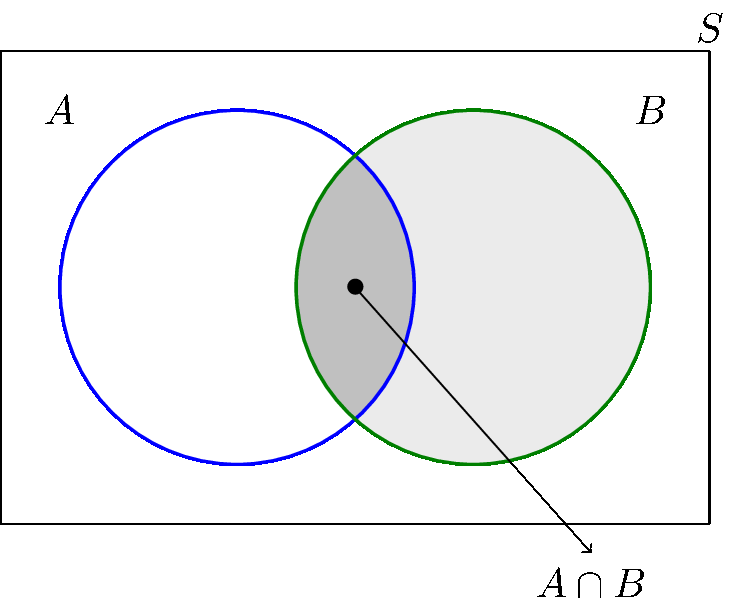
\includegraphics[width=0.7\linewidth]{figures/conditional_b.png}
\caption{Graphical representation of conditional probability (the gray shaded area).}
\end{figure}

Going back to the hazard rate ($\lambda$) we can now compute the instantaneous default probability conditional to no previous default 

%\[\lambda(t) = \cfrac{\mathbb{P}(A\cap B)}{\mathbb{P}(B)} = \cfrac{\cfrac{DP(\tau\in (t, t+dt))}{dt}}{DP(\tau>t)} = \cfrac{\cfrac{d[1-N(t_0, t)]}{dt}}{N(t_0, t)} = -\cfrac{dN(t_0, t)}{dt}\cdot\frac{1}{N(t_0, t)}\]
\begin{equation}\lambda(t) = \cfrac{P(A\cap B)}{P(B)} = \cfrac{\cfrac{DP(t, t+dt)}{dt}}{DP(t, +\infty)} = \cfrac{\cfrac{d[1-N(t_0, t)]}{dt}}{N(t_0, t)} = -\cfrac{dN(t_0, t)}{dt}\cdot\frac{1}{N(t_0, t)}\end{equation}
where $N$ and $DP$ are survival and default probabilities.% and $\tau$ indicates the time at which the credit event occurred.
Also remember that $DP(t_0, t) = 1 - N(t_0, t)$ or that the probability of default at $t$ is equal to 1 minus the non-default probability.
Conversely, given the hazard rate, the non-default probability can be
determined as:

\begin{equation}
\begin{gathered}
\lambda(t) = -\cfrac{1}{dt}\cdot\cfrac{dN(t_0, t)}{N(t_0, t)} = -\cfrac{d(\textrm{log}N(t_0, t))}{dt} \implies d(\textrm{log}N(t_0, t)) = -\lambda dt\\
N(t_0, t) = \mathrm{exp}\left(-\int_{t_0}^{t}\lambda(s) ds\right)
\end{gathered}
\end{equation}

\subsection{\texttt{CreditCurve} class}

In this Section we develop a \texttt{CreditCurve} class which will be characterized by a list of pillar dates and a corresponding list of non-default probabilities. It has also methods to compute survival probabilities at arbitrary date by interpolation and the hazard rate.
  
\begin{tcolorbox}[breakable, size=fbox, boxrule=1pt, pad at break*=1mm,colback=cellbackground, colframe=cellborder]
\begin{Verbatim}[commandchars=\\\{\}]
\PY{k+kn}{import} \PY{n+nn}{math}
\PY{k+kn}{import} \PY{n+nn}{numpy}

\PY{k}{class} \PY{n+nc}{CreditCurve}\PY{p}{:}
    \PY{k}{def} \PY{n+nf}{\PYZus{}\PYZus{}init\PYZus{}\PYZus{}}\PY{p}{(}\PY{n+nb+bp}{self}\PY{p}{,} \PY{n}{pillar\PYZus{}dates}\PY{p}{,} \PY{n}{ndps}\PY{p}{)}\PY{p}{:}    
        \PY{n+nb+bp}{self}\PY{o}{.}\PY{n}{pillar\PYZus{}dates} \PY{o}{=} \PY{n}{pillar\PYZus{}dates}
        \PY{n+nb+bp}{self}\PY{o}{.}\PY{n}{pillar\PYZus{}days} \PY{o}{=} \PY{p}{[}
            \PY{p}{(}\PY{n}{pd} \PY{o}{\PYZhy{}} \PY{n}{pillar\PYZus{}dates}\PY{p}{[}\PY{l+m+mi}{0}\PY{p}{]}\PY{p}{)}\PY{o}{.}\PY{n}{days}
            \PY{k}{for} \PY{n}{pd} \PY{o+ow}{in} \PY{n}{pillar\PYZus{}dates}
        \PY{p}{]}
        \PY{n+nb+bp}{self}\PY{o}{.}\PY{n}{ndps} \PY{o}{=} \PY{n}{ndps}
        
    \PY{k}{def} \PY{n+nf}{ndp}\PY{p}{(}\PY{n+nb+bp}{self}\PY{p}{,} \PY{n}{value\PYZus{}date}\PY{p}{)}\PY{p}{:}
        \PY{n}{value\PYZus{}days} \PY{o}{=} \PY{p}{(}\PY{n}{value\PYZus{}date} \PY{o}{\PYZhy{}} \PY{n+nb+bp}{self}\PY{o}{.}\PY{n}{pillar\PYZus{}dates}\PY{p}{[}\PY{l+m+mi}{0}\PY{p}{]}\PY{p}{)}\PY{o}{.}\PY{n}{days}
        \PY{k}{return} \PY{n}{interp}\PY{p}{(}\PY{n}{value\PYZus{}days}\PY{p}{,}
                      \PY{n+nb+bp}{self}\PY{o}{.}\PY{n}{pillar\PYZus{}days}\PY{p}{,}
                      \PY{n+nb+bp}{self}\PY{o}{.}\PY{n}{ndps}\PY{p}{)}
    
    \PY{k}{def} \PY{n+nf}{hazard}\PY{p}{(}\PY{n+nb+bp}{self}\PY{p}{,} \PY{n}{value\PYZus{}date}\PY{p}{)}\PY{p}{:}
        \PY{n}{ndp\PYZus{}1} \PY{o}{=} \PY{n+nb+bp}{self}\PY{o}{.}\PY{n}{ndp}\PY{p}{(}\PY{n}{value\PYZus{}date}\PY{p}{)}
        \PY{n}{ndp\PYZus{}2} \PY{o}{=} \PY{n+nb+bp}{self}\PY{o}{.}\PY{n}{ndp}\PY{p}{(}\PY{n}{value\PYZus{}date} \PY{o}{+} \PY{n}{relativedelta}\PY{p}{(}\PY{n}{days}\PY{o}{=}\PY{l+m+mi}{1}\PY{p}{)}\PY{p}{)}
        \PY{n}{delta\PYZus{}t} \PY{o}{=} \PY{l+m+mf}{1.0} \PY{o}{/} \PY{l+m+mf}{365.0}
        \PY{n}{h} \PY{o}{=} \PY{o}{\PYZhy{}}\PY{l+m+mf}{1.0} \PY{o}{/} \PY{n}{ndp\PYZus{}1} \PY{o}{*} \PY{p}{(}\PY{n}{ndp\PYZus{}2} \PY{o}{\PYZhy{}} \PY{n}{ndp\PYZus{}1}\PY{p}{)} \PY{o}{/} \PY{n}{delta\PYZus{}t}
        \PY{k}{return} \PY{n}{h}
\end{Verbatim}
\end{tcolorbox}    

Let's test the newly created class with some inputs.
\begin{tcolorbox}[breakable, size=fbox, boxrule=1pt, pad at break*=1mm,colback=cellbackground, colframe=cellborder]
\begin{Verbatim}[commandchars=\\\{\}]
\PY{k+kn}{from} \PY{n+nn}{datetime} \PY{k}{import} \PY{n}{date}
\PY{k+kn}{from} \PY{n+nn}{dateutil}\PY{n+nn}{.}\PY{n+nn}{relativedelta} \PY{k}{import} \PY{n}{relativedelta}

\PY{n}{start\PYZus{}date = date(2020, 11, 4)}        
\PY{n}{cc} \PY{o}{=} \PY{n}{CreditCurve}\PY{p}{(}
      \PY{p}{[}\PY{n}{start\PYZus{}date}\PY{p}{,} \PY{n}{start\PYZus{}date} \PY{o}{+} \PY{n}{relativedelta}\PY{p}{(}\PY{n}{years}\PY{o}{=}\PY{l+m+mi}{2}\PY{p}{)}\PY{p}{]}\PY{p}{,}
      \PY{p}{[}\PY{l+m+mf}{1.0}\PY{p}{,} \PY{l+m+mf}{0.8}\PY{p}{]}
\PY{p}{)}

\PY{n}{cc}\PY{o}{.}\PY{n}{ndp}\PY{p}{(}\PY{n}{start\PYZus{}date} \PY{o}{+} \PY{n}{relativedelta}\PY{p}{(}\PY{n}{years}\PY{o}{=}\PY{l+m+mi}{1}\PY{p}{)}\PY{p}{)}

0.9
\PY{n}{cc}\PY{o}{.}\PY{n}{hazard}\PY{p}{(}\PY{n}{start\PYZus{}date} \PY{o}{+} \PY{n}{relativedelta}\PY{p}{(}\PY{n}{years}\PY{o}{=}\PY{l+m+mi}{1}\PY{p}{)}\PY{p}{)}

0.1111111114199
\end{Verbatim}
\end{tcolorbox}    
            
\section{Credit Default Swaps}\label{credit-deafult-swaps}

Once we have implemented a \texttt{CreditCurve} class which allows us to
interpolate survival probabilities and also to calculate the hazard rate at arbitrary
dates, we can use it to price \textbf{Credit Default Swaps} (CDSs).

A Credit Default Swap is a financial agreement that the seller of the CDS will compensate the buyer in the event of a debt default or other credit event. 
That is, the seller of the CDS insures the buyer against some reference asset defaulting. The buyer of the CDS makes a series of payments (the CDS \emph{spread}) to the seller and, in exchange, may expect to receive a payoff if the asset defaults.

\subsection{Valuation of CDS (Probability Model)}

Credit default swaps are made up of two legs:

\begin{itemize}
\tightlist
\item
  the \emph{premium} leg: which pays the spread \(S\) periodically until a credit event occurs;
\item
  the \emph{default} leg: which pays \(L = F(1 - R)\), known as the
  \textbf{loss given default} (LGD) if and when the credit event occurs, ($F$ is the notional of the contract, $R$ is the \textbf{recovery value}).
\end{itemize}

\subsubsection{Premium leg}\label{premium-leg}

In the calculation of the premium leg, we'll use the following notation:

\begin{itemize}
\tightlist
\item
  \(d\) today's date;
\item
  \(d_0\) the start date of the CDS (could be different from today's date);
\item
  \(d_1, ..., d_n\) the payment dates of the premium leg, which occur at
  a n-month frequency. We assume that \(d_n\) is the end date of the CDS;
\item
  \(D(d')\) the discount factor between \(d\) and \(d'\);
\item
  \(N(d, d')\) the survival probability between \(d\) and \(d'\);
\item
  \(\tau\) the \emph{random variable} representing the date of the credit event.
\end{itemize}

At each payment date \(d_i\), a cash flow of \(S\) is paid if and only if the
credit event has \emph{not} occurred before that date. Therefore the NPV of the
each flow is

\begin{equation}
f_{\textrm{premium}}^i = \mathbb{E}\left[F\times S \times D(d_i) \times \mathbb{1}(\tau > d_i) \right]\end{equation}
where \(\mathbb{1}(\tau > d_i)\) means that the expectation value has to
be evaluated when \(\tau > d_i\). 

Remembering the definition of expected value~\ref{sec:expected-value), we can interpret 
\(F\cdot S\cdot D(d_i)\) as our variables and \(N(d, d_i)\) as our probabilities so the NPV of the
leg can be expressed as:

\begin{equation}
	\textrm{NPV}_{premium} = F\cdot \sum_{i=1}^{n} S \cdot D(d_i) \cdot N(d, d_i)
\end{equation}

\subsubsection{Default leg}\label{default-leg}

Concerning the default leg, as soon as a credit event occurs (at a time $\tau$) the LGD \(F(1-R)\) is paid out on the same date, i.e. it can potentially be paid on any date between \(d_0\) and \(d_n\). Mathematically, therefore, the NPV of the default leg can be expressed as follows:

\begin{equation}
\mathrm{NPV_{default}} =\mathbb{E}[F(1-R) \times D(\tau) \times \mathbb{1} \{\tau \leq d_n\} ]
\end{equation}

Also in this case we are dealing with a probabilistic event so the expectation value has to be computed taking into account the payments $F(1-R)\times D(\tau)$ averaged over the default probability space $DP(d, \tau)$. 

Using the law of total probability, we can break the previous expression down into the sum
of "daily NPVs" calculated as a function of the \emph{daily} default
probabilities:

\begin{align}
\begin{split}
\mathrm{NPV_{default}} &= \mathbb{E}[F(1-R) \times D(\tau) \times \mathbb{1}\{\tau \leq d_n\} ] \\
&= \sum_{d'=d_0}^{d_n} F(1-R) \times D(\tau = d') DP(d, \tau = d') \\
&= F(1-R) \sum_{d'=d_0}^{d_n} D(d') \left(DP(\tau \geq d') - DP( \tau \geq d'+1) \right) \\
&= F(1-R) \sum_{d'=d_0}^{d_n} D(d') \left( N(d, d') - N(d, d'+1) \right)
\end{split}
\end{align}
where the last step holds since $DP(\tau\geq d^{'}) = 1 - DP(\tau < d^{'}) = 1 - (1-N(d, d^{'})) = N(d, d^{'})$. 
Figure~\ref{fig:default_p} illustrates graphically the step to convert the daily default probability $DP(\tau=d')$.

\begin{figure}[htb]
	\centering
	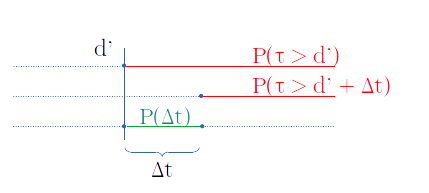
\includegraphics[width=0.7\textwidth]{figures/timeline.png}
	\caption{The probability that a default occurs at a time $\tau = d'+\Delta t$ is equivalent to the default probability at $\tau > d'$ minus the default probability at $\tau>d'+\Delta t$.}
	\label{fig:default_p}
\end{figure}

\subsection{\texttt{CreditDefaultSwap} Class}

As for the other kind of contracts a \texttt{CreditDefaultSwap} class is developed in this Section. In this case the class has methods to compute NPVs for the premium and default legs.

\begin{tcolorbox}[breakable, size=fbox, boxrule=1pt, pad at break*=1mm,colback=cellbackground, colframe=cellborder]
\begin{Verbatim}[commandchars=\\\{\}]
\PY{k+kn}{from} \PY{n+nn}{finmarkets} \PY{k}{import} \PY{n}{generate\PYZus{}swap\PYZus{}dates}
        
\PY{k}{class} \PY{n+nc}{CreditDefaultSwap}\PY{p}{:}
    \PY{k}{def} \PY{n+nf}{\PYZus{}\PYZus{}init\PYZus{}\PYZus{}}\PY{p}{(}\PY{n+nb+bp}{self}\PY{p}{,} \PY{n}{notional}\PY{p}{,} \PY{n}{start\PYZus{}date}\PY{p}{,} \PY{n}{fixed\PYZus{}spread}\PY{p}{,} 
                 \PY{n}{maturity_y}\PY{p}{,} \PY{n}{tenor}\PY{o}{=}\PY{l+m+mf}{3}\PY{p}{,} \PY{n}{recovery}\PY{o}{=}\PY{l+m+mf}{0.4}\PY{p}{)}\PY{p}{:}
        \PY{n+nb+bp}{self}\PY{o}{.}\PY{n}{notional} \PY{o}{=} \PY{n}{notional}
        \PY{n+nb+bp}{self}\PY{o}{.}\PY{n}{payment\PYZus{}dates} \PY{o}{=} \PY{n}{generate\PYZus{}swap\PYZus{}dates}\PY{p}{(}\PY{n}{start\PYZus{}date}\PY{p}{,} 
                                                 \PY{n}{maturity_y}\PY{o}{*}\PY{l+m+mi}{12}\PY{p}{,} \PY{n}{tenor}\PY{p}{)}
        \PY{n+nb+bp}{self}\PY{o}{.}\PY{n}{fixed\PYZus{}spread} \PY{o}{=} \PY{n}{fixed\PYZus{}spread}
        \PY{n+nb+bp}{self}\PY{o}{.}\PY{n}{recovery} \PY{o}{=} \PY{n}{recovery}
    
    \PY{k}{def} \PY{n+nf}{npv\PYZus{}premium\PYZus{}leg}\PY{p}{(}\PY{n+nb+bp}{self}\PY{p}{,} \PY{n}{discount\PYZus{}curve}\PY{p}{,} \PY{n}{credit\PYZus{}curve}\PY{p}{)}\PY{p}{:}
        \PY{n}{npv} \PY{o}{=} \PY{l+m+mi}{0}
        \PY{k}{for} \PY{n}{i} \PY{o+ow}{in} \PY{n+nb}{range}\PY{p}{(}\PY{l+m+mi}{1}\PY{p}{,} \PY{n+nb}{len}\PY{p}{(}\PY{n+nb+bp}{self}\PY{o}{.}\PY{n}{payment\PYZus{}dates}\PY{p}{)}\PY{p}{)}\PY{p}{:}
            \PY{n}{npv} \PY{o}{+}\PY{o}{=} \PY{p}{(}
                \PY{n+nb+bp}{self}\PY{o}{.}\PY{n}{fixed\PYZus{}spread} \PY{o}{*}
                \PY{n}{discount\PYZus{}curve}\PY{o}{.}\PY{n}{df}\PY{p}{(}\PY{n+nb+bp}{self}\PY{o}{.}\PY{n}{payment\PYZus{}dates}\PY{p}{[}\PY{n}{i}\PY{p}{]}\PY{p}{)} \PY{o}{*}
                \PY{n}{credit\PYZus{}curve}\PY{o}{.}\PY{n}{ndp}\PY{p}{(}\PY{n+nb+bp}{self}\PY{o}{.}\PY{n}{payment\PYZus{}dates}\PY{p}{[}\PY{n}{i}\PY{p}{]}\PY{p}{)}
            \PY{p}{)}
        \PY{k}{return} \PY{n}{npv} \PY{o}{*} \PY{n+nb+bp}{self}\PY{o}{.}\PY{n}{notional}
    
    \PY{k}{def} \PY{n+nf}{npv\PYZus{}default\PYZus{}leg}\PY{p}{(}\PY{n+nb+bp}{self}\PY{p}{,} \PY{n}{discount\PYZus{}curve}\PY{p}{,} \PY{n}{credit\PYZus{}curve}\PY{p}{)}\PY{p}{:}
        \PY{n}{npv} \PY{o}{=} \PY{l+m+mi}{0}
        \PY{n}{d} \PY{o}{=} \PY{n+nb+bp}{self}\PY{o}{.}\PY{n}{payment\PYZus{}dates}\PY{p}{[}\PY{l+m+mi}{0}\PY{p}{]}
        
        \PY{k}{while} \PY{n}{d} \PY{o}{\PYZlt{}}\PY{o}{=} \PY{n+nb+bp}{self}\PY{o}{.}\PY{n}{payment\PYZus{}dates}\PY{p}{[}\PY{o}{\PYZhy{}}\PY{l+m+mi}{1}\PY{p}{]}\PY{p}{:}
            \PY{n}{npv} \PY{o}{+}\PY{o}{=} \PY{n}{discount\PYZus{}curve}\PY{o}{.}\PY{n}{df}\PY{p}{(}\PY{n}{d}\PY{p}{)} \PY{o}{*} \PY{p}{(}
                \PY{n}{credit\PYZus{}curve}\PY{o}{.}\PY{n}{ndp}\PY{p}{(}\PY{n}{d}\PY{p}{)} \PY{o}{\PYZhy{}}
                \PY{n}{credit\PYZus{}curve}\PY{o}{.}\PY{n}{ndp}\PY{p}{(}\PY{n}{d} \PY{o}{+} \PY{n}{relativedelta}\PY{p}{(}\PY{n}{days}\PY{o}{=}\PY{l+m+mi}{1}\PY{p}{)}\PY{p}{)}
            \PY{p}{)}
            \PY{n}{d} \PY{o}{+}\PY{o}{=} \PY{n}{relativedelta}\PY{p}{(}\PY{n}{days}\PY{o}{=}\PY{l+m+mi}{1}\PY{p}{)}
        \PY{k}{return} \PY{n}{npv} \PY{o}{*} \PY{n+nb+bp}{self}\PY{o}{.}\PY{n}{notional} \PY{o}{*} \PY{p}{(}\PY{l+m+mi}{1} \PY{o}{\PYZhy{}} \PY{n+nb+bp}{self}\PY{o}{.}\PY{n}{recovery}\PY{p}{)}
    
    \PY{k}{def} \PY{n+nf}{npv}\PY{p}{(}\PY{n+nb+bp}{self}\PY{p}{,} \PY{n}{discount\PYZus{}curve}\PY{p}{,} \PY{n}{credit\PYZus{}curve}\PY{p}{)}\PY{p}{:}
        \PY{k}{return} \PY{n+nb+bp}{self}\PY{o}{.}\PY{n}{npv\PYZus{}default\PYZus{}leg}\PY{p}{(}\PY{n}{discount\PYZus{}curve}\PY{p}{,} \PY{n}{credit\PYZus{}curve}\PY{p}{)} \PY{o}{\PYZhy{}} \PYZbs{}
               \PY{n+nb+bp}{self}\PY{o}{.}\PY{n}{npv\PYZus{}premium\PYZus{}leg}\PY{p}{(}\PY{n}{discount\PYZus{}curve}\PY{p}{,} \PY{n}{credit\PYZus{}curve}\PY{p}{)}
\end{Verbatim}
\end{tcolorbox}    

To test the class data contained in \href{https://drive.google.com/file/d/1mugHyet3H9tcSAvYvt8G4_kpfaEbVY7b/view?usp=sharing}{discount\_curve\_ch10.xlsx} is used.

\begin{tcolorbox}[breakable, size=fbox, boxrule=1pt, pad at break*=1mm,colback=cellbackground, colframe=cellborder]
\begin{Verbatim}[commandchars=\\\{\}]
\PY{k+kn}{import} \PY{n+nn}{pandas} \PY{k}{as} \PY{n+nn}{pd}
	
\PY{k+kn}{from} \PY{n+nn}{datetime} \PY{k}{import} \PY{n}{date}
\PY{k+kn}{from} \PY{n+nn}{dateutil}\PY{n+nn}{.}\PY{n+nn}{relativedelta} \PY{k}{import} \PY{n}{relativedelta}
\PY{k+kn}{from} \PY{n+nn}{finmarkets} \PY{k}{import} \PY{n}{DiscountCurve}
	
\PY{n}{dc\PYZus{}data} \PY{o}{=} \PY{n}{pd}\PY{o}{.}\PY{n}{read\PYZus{}excel}\PY{p}{(}\PY{l+s+s2}{\PYZdq{}}\PY{l+s+s2}{discount\PYZus{}curve\PYZus{}ch10.xlsx}\PY{l+s+s2}{\PYZdq{}}\PY{p}{)}

\PY{n}{observation\PYZus{}date = date(2020, 11, 1)}        
\PY{n}{dc} \PY{o}{=} \PY{n}{DiscountCurve}\PY{p}{(}\PY{n}{observation\PYZus{}date}\PY{p}{,} 
\PY{n}{dc\PYZus{}data}\PY{p}{[}\PY{l+s+s1}{\PYZsq{}}\PY{l+s+s1}{pillars}\PY{l+s+s1}{\PYZsq{}}\PY{p}{]}\PY{o}{.}\PY{n}{dt}\PY{o}{.}\PY{n}{date}\PY{o}{.}\PY{n}{tolist}\PY{p}{(}\PY{p}{)}\PY{p}{,}
\PY{n}{dc\PYZus{}data}\PY{p}{[}\PY{l+s+s1}{\PYZsq{}}\PY{l+s+s1}{discount\PYZus{}factors}\PY{l+s+s1}{\PYZsq{}}\PY{p}{]}\PY{o}{.}\PY{n}{tolist}\PY{p}{(}\PY{p}{)}\PY{p}{)}

\PY{n}{credit\PYZus{}curve} \PY{o}{=} \PY{n}{CreditCurve}\PY{p}{(}\PY{p}{[}\PY{n}{start\PYZus{}date}\PY{p}{,} 
                           \PY{n}{start\PYZus{}date} \PY{o}{+} \PY{n}{relativedelta}\PY{p}{(}\PY{n}{months}\PY{o}{=}\PY{l+m+mi}{36}\PY{p}{)}\PY{p}{]}\PY{p}{,} 
                           \PY{p}{[}\PY{l+m+mf}{1.0}\PY{p}{,} \PY{l+m+mf}{0.7}\PY{p}{]}\PY{p}{)}

\PY{n}{cds} \PY{o}{=} \PY{n}{CreditDefaultSwap}\PY{p}{(}\PY{l+m+mf}{1e6}\PY{p}{,} \PY{n}{start\PYZus{}date}\PY{p}{,} \PY{l+m+mf}{0.03}\PY{p}{,} \PY{l+m+mi}{3}\PY{p}{)}
\PY{n}{cds}\PY{o}{.}\PY{n}{premium\PYZus{}leg\PYZus{}npv}\PY{p}{(}\PY{n}{dc}\PY{p}{,} \PY{n}{credit\PYZus{}curve}\PY{p}{)}

303058.4667954984
\end{Verbatim}
\end{tcolorbox}

\begin{tcolorbox}[breakable, size=fbox, boxrule=1pt, pad at break*=1mm,colback=cellbackground, colframe=cellborder]
\begin{Verbatim}[commandchars=\\\{\}]
\PY{n}{cds}\PY{o}{.}\PY{n}{default\PYZus{}leg\PYZus{}npv}\PY{p}{(}\PY{n}{dc}\PY{p}{,} \PY{n}{credit\PYZus{}curve}\PY{p}{)}

180888.9540606495
\end{Verbatim}
\end{tcolorbox}

\begin{tcolorbox}[breakable, size=fbox, boxrule=1pt, pad at break*=1mm,colback=cellbackground, colframe=cellborder]
\begin{Verbatim}[commandchars=\\\{\}]
\PY{n}{cds}\PY{o}{.}\PY{n}{npv}\PY{p}{(}\PY{n}{dc}\PY{p}{,} \PY{n}{credit\PYZus{}curve}\PY{p}{)}

-122169.51273484889
\end{Verbatim}
\end{tcolorbox}
	
\subsection{Break-even Spread}
The break-even spread of a credit default swap is the value of the fixed rate paid in the premium leg that makes the CDS net present value 0.

In this Section a new method to compute the break-even spread of a CDS will be added to the \texttt{CreditDefaultSwap} class.

To determine the break-even spread is enough to impose that the NPV of the premium and default legs are equal:

\begin{equation}
S \cdot\sum_{i=1}^{n} D(d_i) \cdot N(d, d_i)
= (1-R) \sum_{d'=d_0}^{d_n} D(d') \left( N(d, d') - N(d, d'+1) \right)
\end{equation}
solving for $S$ we obtained the wanted spread

\begin{equation}
S_{\mathrm{breakeven}} = \cfrac{(1-R) \sum_{d'=d_0}^{d_n} D(d') \left( N(d, d') - N(d, d'+1) \right)}{\sum_{i=1}^{n} D(d_i) \cdot N(d, d_i)}
\end{equation}

The implementation is relatively easy:

\begin{tcolorbox}[breakable, size=fbox, boxrule=1pt, pad at break*=1mm,colback=cellbackground, colframe=cellborder]
\begin{Verbatim}[commandchars=\\\{\}]
  \PY{k}{def} \PY{n+nf}{breakevenRate}\PY{p}{(}\PY{n+nb+bp}{self}\PY{p}{,} \PY{n}{discount\PYZus{}curve}\PY{p}{,} \PY{n}{credit\PYZus{}curve}\PY{p}{)}\PY{p}{:}
    \PY{n}{num} \PY{o}{=} \PY{n+nb+bp}{self}\PY{o}{.}\PY{n}{npv\PYZus{}default\PYZus{}leg}\PY{p}{(}\PY{n}{discount\PYZus{}curve}\PY{p}{,} \PY{n}{credit\PYZus{}curve}\PY{p}{)}
    \PY{n}{den} \PY{o}{=} \PY{n+nb+bp}{self}\PY{o}{.}\PY{n}{npv\PYZus{}premium\PYZus{}leg}\PY{p}{(}\PY{n}{discount\PYZus{}curve}\PY{p}{,} \PY{n}{credit\PYZus{}curve}\PY{p}{)}\PY{o}{/}\PY{n+nb+bp}{self}\PY{o}{.}\PY{n}{fixed\PYZus{}spread}
    \PY{k}{return} \PY{n}{num}\PY{o}{/}\PY{n}{den}
\end{Verbatim}
\end{tcolorbox}

\section{Credit Ratings}\label{credit-ratings}

A credit rating is a quantified assessment of the creditworthiness of a
borrower either in general terms or with respect to a particular debt or
financial obligation. A credit rating can be assigned to any entity that
seeks to borrow money (e.g. an individual, corporation, state or
provincial authority, or sovereign government).

A loan is a essentially a promise and the credit rating determines the
likelihood that the borrower will be able to pay back it within the loan
agreement terms. A high credit rating indicates a high possibility of
paying back the loan in its entirety without any issues; a poor credit
rating suggests that the borrower has had trouble paying back loans in
the past and might follow the same pattern in the future.

Individual credit is scored from credit bureaus (e.g. Experian and
TransUnion) and it is reported as a number, generally ranging from 300
to 850.

Credit assessment and evaluation for companies and governments instead
is generally done by credit rating agencies (e.g. Standard \& Poor's
(S\&P), Moody's, or Fitch), which typically assign letter grades to
indicate ratings. Standard \& Poor's, for instance, has a credit rating
scale ranging from AAA (excellent) to C and D. A debt instrument with a
rating below BB is considered to be a speculative grade or a junk bond,
which means it is more likely to default on loans.

\subsection{Why Credit Ratings Are Important}\label{why-credit-ratings-are-important}

A borrowing entity will strive to have the highest possible credit
rating since it has a major impact on interest rates charged by lenders.
Rating agencies, on the other hand, must take a balanced and objective
view of the borrower's financial situation and capacity to service/repay
the debt.

A credit rating not only determines whether or not a borrower will be
approved for a loan but also determines the interest rate at which the
loan will need to be repaid. Since companies depend on loans for many
expenses, being denied a loan could spell disaster, and
in any case a high interest rate is much more difficult to pay back.
Credit ratings also play a large role in a potential investor's
determining whether or not to purchase bonds. A poor credit rating is a
risky investment; it indicates a larger probability that the company
will be unable to make its bond payments.

It is important for a borrower to remain diligent in maintaining a high
credit rating. Credit ratings are never static; in fact, they change all
the time based on the newest data, and one negative debt will bring down
even the best score. 
Credit also takes time to build up. An entity with
good credit but a short credit history is not seen as positively as
another entity with the same quality of credit but a longer history.
Debtors want to know a borrower can maintain good credit consistently
over time.

\section{Determine Default Probabilities from Market Quotes}
In this Section we will see how we can derive default probabilities implied by market quotes. We will derive them both from bonds and credit default swaps.

\subsection{Bonds}\label{bonds}

A bond is an instrument that represents a loan made by an investor to a
borrower (typically corporate or governmental). Bonds are used by
companies, municipalities, states, and sovereign governments to finance
projects and operations. 

Owners of bonds are debt-holders, or creditors,
of the issuer. Bond details include the end date (when the principal of
the loan is due to be paid to the bond owner) and usually includes the
terms for variable or fixed interest payments made by the borrower.

The \emph{coupon} is the interest rate that the issuer pays to the holder.
This rate can be fixed throughout the life of the bond but it can also
vary with a money market index, such as LIBOR, or it can be even more
exotic.

\subsection{Valuing a Bond}\label{sec:bond_pricing}

The value of a bond can be computed as the present discounted value of
future cash flows generated by the bond itself.

For example consider a 3-years bond with a face value of \euro{100}
providing coupons at a 6\% rate annually. Assume also that the spot
rates are 5.0\% 5.8\% and 6.4\% for 1, 2, 3 year maturities. To
compute the present value of the first coupon we need to discount it at
5.0\% for 1 year, for the second the discount has to be at 5.8\% and so
on. The value will be then:

\[P_{\mathrm{bond}}=6e^{-0.05\cdot 1}+6e^{-0.058\cdot 2}+106e^{-0.064\cdot 3} = \textrm{\euro{98.53}}\]

\begin{tcolorbox}[breakable, size=fbox, boxrule=1pt, pad at break*=1mm,colback=cellbackground, colframe=cellborder]
\begin{Verbatim}[commandchars=\\\{\}]
\PY{k+kn}{from} \PY{n+nn}{math} \PY{k}{import} \PY{n}{exp}
\PY{n}{rates} \PY{o}{=} \PY{p}{[}\PY{l+m+mf}{0.05}\PY{p}{,} \PY{l+m+mf}{0.058}\PY{p}{,} \PY{l+m+mf}{0.064}\PY{p}{,} \PY{l+m+mf}{0.068}\PY{p}{]}

\PY{n}{N} \PY{o}{=} \PY{l+m+mi}{100}
\PY{n}{maturity} \PY{o}{=} \PY{l+m+mi}{3}
\PY{n}{fixed\PYZus{}coupon} \PY{o}{=} \PY{l+m+mf}{0.06}
\PY{n}{price} \PY{o}{=} \PY{l+m+mi}{0}
\PY{k}{for} \PY{n}{tau} \PY{o+ow}{in} \PY{n+nb}{range}\PY{p}{(}\PY{l+m+mi}{1}\PY{p}{,} \PY{n}{maturity} \PY{o}{+} \PY{l+m+mi}{1}\PY{p}{)}\PY{p}{:}
    \PY{n}{price} \PY{o}{+}\PY{o}{=} \PY{n}{N} \PY{o}{*} \PY{n}{fixed\PYZus{}coupon} \PY{o}{*} \PY{n}{exp}\PY{p}{(}\PY{o}{\PYZhy{}}\PY{n}{rates}\PY{p}{[}\PY{n}{tau}\PY{o}{\PYZhy{}}\PY{l+m+mi}{1}\PY{p}{]} \PY{o}{*} \PY{n}{tau}\PY{p}{)}

\PY{n}{price} \PY{o}{+}\PY{o}{=} \PY{n}{N} \PY{o}{*} \PY{n}{exp}\PY{p}{(}\PY{o}{\PYZhy{}}\PY{n}{rates}\PY{p}{[}\PY{n}{maturity} \PY{o}{\PYZhy{}} \PY{l+m+mi}{1}\PY{p}{]} \PY{o}{*} \PY{n}{maturity}\PY{p}{)}
    
\PY{n+nb}{print} \PY{p}{(}\PY{l+s+s2}{\PYZdq{}}\PY{l+s+si}{\PYZob{}:.2f\PYZcb{}}\PY{l+s+s2}{ EUR}\PY{l+s+s2}{\PYZdq{}}\PY{o}{.}\PY{n}{format}\PY{p}{(}\PY{n}{price}\PY{p}{)}\PY{p}{)}

98.53 EUR
\end{Verbatim}
\end{tcolorbox}

\subsection{Implied Probability of Default from Coupon Bonds}\label{default-probabilities-and-bond-prices}

The price of a bond issued by a party is directly linked to the credit
rating of that party, since there is always an associated default risk, which means that the borrower might not be able to repay
fully or partially the amount of the taken loan. 

Bonds with low ratings, called junk bonds, are sold at lower prices (since riskier) while those with higher ratings, called investment-grade bonds, are sold at higher prices.

Let's see with an example how the default probability can be determined
from bond prices. Imagine to have a bond and let \(x\) represent the
present value of a bond cash flow stream.

When you have a default probability associated to the issuer to valuate
the bond we need to take each possible value of \(x\), multiply it by
its probability and sum the results. In other words the value of the
bond should equal the mathematical expectation of \(x\).

Consider a bond which pays \(F\) at maturity and that the issuer of this
bond has a default probability \(P\) (in case of default the recovery is
\(R\)).What will be the price of this bond ?

\begin{equation}
V_{bond} =
\begin{cases}
& D \cdot R \cdot F\quad\textrm{(in case of default of the issuer)}\\
&D \cdot F\quad\textrm{(in case of no default)}\\
\end{cases}\end{equation} 
where \(D\) is the proper discount factor. Since we don't
know if the issuer will default or not we can estimate the bond price as

\begin{equation}
V_{bond} = D \cdot R \cdot F \cdot DP ( \tau ) + D \cdot F \cdot ( 1 − DP ( \tau)) = D\cdot F \cdot ( 1 − ( 1 − R ) DP ( \tau ))\end{equation}

From the this equation is clear that the higher the default probability
the lower is the bond price. Conversely, given the market price of the
bond we can estimate the issuer default probability.

%The probability of a company default can be estimated directly from
%the prices of its issued bonds. Imagine that the spread $s$
%between a corporate bond over the risk-free rate should compensate for
%the losses in case of default, so naively:
%
%\[\lambda = \frac{s}{1-R}\]
%where $\lambda$ is the annualised hazard rate and $R$ the recovery rate.

In a more detailed way let $X$ represent the present value of a bond cash flow stream. When you
have a default probability then $X$ becomes a random variable with a range
of possible values. The way
to value the bond in this case is to take each possible value of $X$, multiply it
by its probability and sum the results. In other words the value of the bond
should equal the mathematical expectation of $X$.

To illustrate the idea, consider the case of a bond with 4 coupon payments
until maturity. Let $S$ be the probability that the bond \emph{survives} from one
coupon payment to the next and let $X_i$ ($i$ = 0, 1, 2, 3, 4) be the value of
$X$ given that the bond defaults after making its $i$-th coupon payment. 
The expectation of $X$ can then be expressed as:

\begin{align}
\begin{split}
\mathbb{E}(X) &= X_0(1-S) + X_1 S(1-S) + X_2 S^2 (1-S) + X_3 S^3 (1-S) + X_4 S^4 \\
&= X_0 + (X_1 - X_0)S + (X_2 - X_1)S^2 + (X_3 - X_2)S^3 + (X_4 - X_3)S^4
\end{split}
\end{align}

Assuming a constant recovery value $R$ the values $X_i$ are:

\begin{align}
\begin{split}
X_0 &= RF \\
X_1 &= (C + RF)\cdot D \\
X_2 &= C\cdot D + (C + RF)\cdot D^2 \\
X_3 &= C\cdot D + C\cdot D^2 + (C + RF)\cdot D^3 \\
X_4 &= C\cdot D + C\cdot D^2 + C\cdot D^3 + (C + F)\cdot D^4 \\
\end{split}
\end{align}
where $D$ represent the proper discount factor and $F$ the bond face value.
Substituting into the expectation formula:

\begin{align}
\begin{split}
\mathbb{E}(X) &= C((SD) + (SD)^2 + (SD)^3 + (SD)^4) + \\
&RF(1-S)(1+(SD)+(SD)^2 + (SD)^3) + F(SD)^4 
\end{split}
\end{align}

It is now easy to generalize to the case of $N$ coupons:

\begin{equation} \mathbb{E}(X) = C \sum_{k=1}^{N}{(SD)^k} + RF(1-S)\sum_{k=1}^{N-1}{(SD)^k} + F(SD)^N \end{equation}

Each of the sums in this s formula is a geometric series that can be collapsed
into a single term. The formula for collapsing a general geometric series is 

\begin{equation}\sum_{k=0}^N a^k = 1 + a + a^2 + \ldots + a^N = \cfrac{1-a^{N+1}}{1-a} \end{equation}

Hence we get:

\begin{align}
\begin{split}
\mathbb{E}(X) &= (CSD) \cfrac{1-(SD)^N}{1-(SD)}+RF(1-S)\cfrac{1-(SD)^N}{1-(SD)} + F(SD)^N \\
&= \Big(CSD + RF(1-S)\Big)\cfrac{1-(SD)^N}{1-(SD)} + F(SD)^N 
\end{split}
\end{align}

With $\mathbb{E}(X)$ equal to the price of the bond, this equation can be solved numerically for the survival probability $S$.

To get the default probability for the bond, simply subtract the survival
probability from 1. The cumulative default probability, or the probability that the bond defaults anytime within the next $k$ coupon periods is $(1 - S^k)$.

There are several ways to test the formula for logical consistency. First look
at the case where the survival probability is zero so that with $S = 0$ the
formula reduces to:

\begin{equation}\mathbb{E}(X) = RF\end{equation}
this is logical since when default is immanent the price should just equal the
recovery amount.
In the case where survival is certain and the risk free rate is zero you have
$S = 1$ and $D=1$:

\begin{equation}\mathbb{E}(X) = NC + F \end{equation}
The price here is equal to the total of the coupon payments plus the face
value, as you would expect.

Next an example with a \texttt{python} implementation which uses \texttt{brentq}.

\begin{tcolorbox}[breakable, size=fbox, boxrule=1pt, pad at break*=1mm,colback=cellbackground, colframe=cellborder]
\begin{Verbatim}[commandchars=\\\{\}]
\PY{k+kn}{from} \PY{n+nn}{scipy}\PY{n+nn}{.}\PY{n+nn}{optimize} \PY{k}{import} \PY{n}{brentq}
	
\PY{n}{C} \PY{o}{=} \PY{l+m+mf}{0.05} \PY{c+c1}{\PYZsh{} coupon}
\PY{n}{r} \PY{o}{=} \PY{l+m+mf}{0.03} \PY{c+c1}{\PYZsh{} risk\PYZhy{}free rate}
\PY{n}{D} \PY{o}{=} \PY{l+m+mi}{1}\PY{o}{/}\PY{p}{(}\PY{l+m+mi}{1}\PY{o}{+}\PY{n}{r}\PY{p}{)} \PY{c+c1}{\PYZsh{} discount factor}
\PY{n}{F}\PY{o}{=}\PY{l+m+mi}{100} \PY{c+c1}{\PYZsh{} bond face value}
\PY{n}{R}\PY{o}{=}\PY{l+m+mf}{0.4} \PY{c+c1}{\PYZsh{} recovery}
\PY{n}{N}\PY{o}{=}\PY{l+m+mi}{4} \PY{c+c1}{\PYZsh{} maturity}
\PY{n}{trading\PYZus{}price} \PY{o}{=} \PY{l+m+mi}{80}
	
\PY{k}{def} \PY{n+nf}{func}\PY{p}{(}\PY{n}{x}\PY{p}{)}\PY{p}{:}
	\PY{c+c1}{\PYZsh{} x survival probability between two coupons}
	\PY{k}{return} \PY{n}{C}\PY{o}{*}\PY{n}{x}\PY{o}{*}\PY{n}{D} \PY{o}{+} \PY{n}{R}\PY{o}{*}\PY{n}{F}\PY{o}{*}\PY{p}{(}\PY{l+m+mi}{1}\PY{o}{\PYZhy{}}\PY{n}{x}\PY{p}{)}\PY{o}{*}\PY{p}{(}\PY{l+m+mi}{1}\PY{o}{\PYZhy{}}\PY{p}{(}\PY{n}{x}\PY{o}{*}\PY{n}{D}\PY{p}{)}\PY{o}{*}\PY{o}{*}\PY{n}{N}\PY{p}{)}\PY{o}{/}\PY{p}{(}\PY{l+m+mi}{1}\PY{o}{\PYZhy{}}\PY{n}{x}\PY{o}{*}\PY{n}{D}\PY{p}{)}\PY{o}{+}\PY{n}{F}\PY{o}{*}\PY{p}{(}\PY{n}{x}\PY{o}{*}\PY{n}{D}\PY{p}{)}\PY{o}{*}\PY{o}{*}\PY{n}{N}\PY{o}{\PYZhy{}}\PY{n}{trading\PYZus{}price}
	
\PY{n}{res} \PY{o}{=} \PY{n}{brentq}\PY{p}{(}\PY{n}{func}\PY{p}{,} \PY{l+m+mi}{0}\PY{p}{,} \PY{l+m+mi}{1}\PY{p}{)}
\PY{n+nb}{print} \PY{p}{(}\PY{l+s+s2}{\PYZdq{}}\PY{l+s+s2}{P\PYZhy{}default before next coupon: }\PY{l+s+si}{\PYZob{}:.1f\PYZcb{}}\PY{l+s+s2}{\PYZpc{}}\PY{l+s+s2}{\PYZdq{}}\PY{o}{.}\PY{n}{format}\PY{p}{(}\PY{p}{(}\PY{l+m+mi}{1}\PY{o}{\PYZhy{}}\PY{n}{res}\PY{p}{)}\PY{o}{*}\PY{l+m+mi}{100}\PY{p}{)}\PY{p}{)}

P-default before next coupon: 4.7\%
\end{Verbatim}
\end{tcolorbox}

\subsection{Implied Probability of Default from CDS}\label{default-probabilities-and-cds}

In order to derive default probabilities from credit default swap market quotes we can exploit the \emph{bootstrap technique}. If we consider again the parallelism between discount and credit curves indeed we can follow the same steps applied in Chapter~\ref{swaps-and-bootstrapping---practical-lesson-5} when deriving the discount factors from overnight index swaps.

Let's summarize the procedure: 
\begin{itemize}
\tightlist
\item create a CDS contracts for each available market quote;
\item implement an objective function to minimize the squared sum of the CDS
	NPVs, the function has to implement also a \texttt{CreditCurve} with
	the unknown (to be determined survival probabilities) and a list of pillars corresponding to the CDS expiry dates;
\item set initial guesses and boundary conditions for the
	unknown parameters (the first survival probability has to be set to 1
	since no default happened !, the others free to move between $[0.01, 1]$ because they are probabilities);
\item using the \texttt{scipy.optimize.minimize} to find the curve.
\end{itemize}

As it is clear those are almost exactly the same steps already seen for the discount factors.

We will now implement again the bootstrapping from the market quotes saved in \href{https://drive.google.com/file/d/1BOtwCFYk0CUwYkMhnowWTj0HNOpBefd_/view?usp=sharing}{cds\_quotes.xlsx} and for the discount curve \href{https://drive.google.com/file/d/1mugHyet3H9tcSAvYvt8G4_kpfaEbVY7b/view?usp=sharing}{discount\_curve\_ch10.xlsx}.

So first load the market data and create a discount curve and the swaps with it.
\begin{tcolorbox}[breakable, size=fbox, boxrule=1pt, pad at break*=1mm,colback=cellbackground, colframe=cellborder]
\begin{Verbatim}[commandchars=\\\{\}]
\PY{k+kn}{import} \PY{n+nn}{pandas} \PY{k}{as} \PY{n+nn}{pd}
\PY{k+kn}{from} \PY{n+nn}{datetime} \PY{k}{import} \PY{n}{date}
\PY{k+kn}{from} \PY{n+nn}{finmarkets} \PY{k}{import} \PY{n}{CreditDefaultSwap}\PY{p}{,} \PY{n}{CreditCurve}\PY{p}{,} \PY{n}{DiscountCurve}
	
\PY{c+c1}{\PYZsh{} load market data}
\PY{n}{dc} \PY{o}{=} \PY{n}{pd}\PY{o}{.}\PY{n}{read\PYZus{}excel}\PY{p}{(}\PY{l+s+s2}{\PYZdq{}}\PY{l+s+s2}{discount\PYZus{}curve\PYZus{}ch10.xlsx}\PY{l+s+s2}{\PYZdq{}}\PY{p}{)}
\PY{n}{mq} \PY{o}{=} \PY{n}{pd}\PY{o}{.}\PY{n}{read\PYZus{}excel}\PY{p}{(}\PY{l+s+s2}{\PYZdq{}}\PY{l+s+s2}{cds\PYZus{}quotes.xlsx}\PY{l+s+s2}{\PYZdq{}}\PY{p}{)}
	
\PY{c+c1}{\PYZsh{} create DiscountCurve}
\PY{n}{discount\PYZus{}curve} \PY{o}{=} \PY{n}{DiscountCurve}\PY{p}{(}\PY{n}{observation\PYZus{}date}\PY{p}{,}
                               \PY{n}{dc}\PY{p}{[}\PY{l+s+s1}{\PYZsq{}}\PY{l+s+s1}{pillars}\PY{l+s+s1}{\PYZsq{}}\PY{p}{]}\PY{o}{.}\PY{n}{dt}\PY{o}{.}\PY{n}{date}\PY{o}{.}\PY{n}{tolist}\PY{p}{(}\PY{p}{)}\PY{p}{,}
                               \PY{n}{dc}\PY{p}{[}\PY{l+s+s1}{\PYZsq{}}\PY{l+s+s1}{discount\PYZus{}factors}\PY{l+s+s1}{\PYZsq{}}\PY{p}{]}\PY{o}{.}\PY{n}{tolist}\PY{p}{(}\PY{p}{)}\PY{p}{)}
	
\PY{n}{cdswaps} \PY{o}{=} \PY{p}{[}\PY{p}{]}
\PY{n}{pillar\PYZus{}dates} \PY{o}{=} \PY{p}{[}\PY{n}{start\PYZus{}date}\PY{p}{]}
\PY{k}{for} \PY{n}{i} \PY{o+ow}{in} \PY{n+nb}{range}\PY{p}{(}\PY{n+nb}{len}\PY{p}{(}\PY{n}{mq}\PY{p}{)}\PY{p}{)}\PY{p}{:}
    \PY{n}{cds} \PY{o}{=} \PY{n}{CreditDefaultSwap}\PY{p}{(}\PY{l+m+mf}{1e6}\PY{p}{,}
                            \PY{n}{start\PYZus{}date}\PY{p}{,}
                            \PY{n}{mq}\PY{p}{[}\PY{l+s+s1}{\PYZsq{}}\PY{l+s+s1}{quote}\PY{l+s+s1}{\PYZsq{}}\PY{p}{]}\PY{o}{.}\PY{n}{tolist}\PY{p}{(}\PY{p}{)}\PY{p}{[}\PY{n}{i}\PY{p}{]}\PY{p}{,}
                            \PY{n}{mq}\PY{p}{[}\PY{l+s+s1}{\PYZsq{}}\PY{l+s+s1}{months}\PY{l+s+s1}{\PYZsq{}}\PY{p}{]}\PY{o}{.}\PY{n}{tolist}\PY{p}{(}\PY{p}{)}\PY{p}{[}\PY{n}{i}\PY{p}{]}\PY{o}{/}\PY{o}{/}\PY{l+m+mi}{12}\PY{p}{)}
    \PY{n}{cdswaps}\PY{o}{.}\PY{n}{append}\PY{p}{(}\PY{n}{cds}\PY{p}{)}
    \PY{n}{pillar\PYZus{}dates}\PY{o}{.}\PY{n}{append}\PY{p}{(}\PY{n}{cds}\PY{o}{.}\PY{n}{payment\PYZus{}dates}\PY{p}{[}\PY{o}{\PYZhy{}}\PY{l+m+mi}{1}\PY{p}{]}\PY{p}{)}
\end{Verbatim}
\end{tcolorbox}

Then the objective function:
\begin{tcolorbox}[breakable, size=fbox, boxrule=1pt, pad at break*=1mm,colback=cellbackground, colframe=cellborder]
\begin{Verbatim}[commandchars=\\\{\}]
\PY{k}{def} \PY{n+nf}{objective\PYZus{}function}\PY{p}{(}\PY{n}{unknown\PYZus{}ndps}\PY{p}{)}\PY{p}{:}
    \PY{n}{credit\PYZus{}curve} \PY{o}{=} \PY{n}{CreditCurve}\PY{p}{(}\PY{n}{pillar\PYZus{}dates}\PY{p}{,} 
                               \PY{n}{unknown\PYZus{}ndps}\PY{p}{)}
	
    \PY{n}{sum\PYZus{}sq} \PY{o}{=} \PY{l+m+mi}{0}
    \PY{k}{for} \PY{n}{cds} \PY{o+ow}{in} \PY{n}{cdswaps}\PY{p}{:}
        \PY{n}{sum\PYZus{}sq} \PY{o}{+}\PY{o}{=} \PY{n}{cds}\PY{o}{.}\PY{n}{npv}\PY{p}{(}\PY{n}{discount\PYZus{}curve}\PY{p}{,} 
                          \PY{n}{credit\PYZus{}curve}\PY{p}{)}\PY{o}{*}\PY{o}{*}\PY{l+m+mi}{2}
    \PY{k}{return} \PY{n}{sum\PYZus{}sq}
\end{Verbatim}
\end{tcolorbox}

The guess values and the boundaries
\begin{tcolorbox}[breakable, size=fbox, boxrule=1pt, pad at break*=1mm,colback=cellbackground, colframe=cellborder]
\begin{Verbatim}[commandchars=\\\{\}]
\PY{n}{ndp\PYZus{}guess} \PY{o}{=} \PY{p}{[}\PY{l+m+mf}{0.01} \PY{k}{for} \PY{n}{\PYZus{}} \PY{o+ow}{in} \PY{n+nb}{range}\PY{p}{(}\PY{n+nb}{len}\PY{p}{(}\PY{n}{pillar\PYZus{}dates}\PY{p}{)}\PY{p}{)}\PY{p}{]}
\PY{n}{bounds} \PY{o}{=} \PY{p}{[}\PY{p}{(}\PY{l+m+mf}{0.01}\PY{p}{,} \PY{l+m+mi}{1}\PY{p}{)} \PY{k}{for} \PY{n}{\PYZus{}} \PY{o+ow}{in} \PY{n+nb}{range}\PY{p}{(}\PY{n+nb}{len}\PY{p}{(}\PY{n}{pillar\PYZus{}dates}\PY{p}{)}\PY{p}{)}\PY{p}{]}
\PY{n}{bounds}\PY{p}{[}\PY{l+m+mi}{0}\PY{p}{]} \PY{o}{=} \PY{p}{(}\PY{l+m+mi}{1}\PY{p}{,} \PY{l+m+mi}{1}\PY{p}{)}
\end{Verbatim}
\end{tcolorbox}

And finally we can run the minimizer
\begin{tcolorbox}[breakable, size=fbox, boxrule=1pt, pad at break*=1mm,colback=cellbackground, colframe=cellborder]
\begin{Verbatim}[commandchars=\\\{\}]
\PY{k+kn}{from} \PY{n+nn}{scipy}\PY{n+nn}{.}\PY{n+nn}{optimize} \PY{k}{import} \PY{n}{minimize}
\PY{n}{r} \PY{o}{=} \PY{n}{minimize}\PY{p}{(}\PY{n}{objective\PYZus{}function}\PY{p}{,} \PY{n}{ndp\PYZus{}guess}\PY{p}{,} \PY{n}{bounds}\PY{o}{=}\PY{n}{bounds}\PY{p}{)}
\PY{n+nb}{print} \PY{p}{(}\PY{n}{r}\PY{p}{)}

fun: 4.046279903873944e-05
hess\_inv: <7x7 LbfgsInvHessProduct with dtype=float64>
jac: array([ 3.68076297e+04,  1.31881916e-01, -2.41176850e-02,
2.79451870e-01,
-1.41296672e-01, -1.14049675e-01, -1.14108073e-01])
message: b'CONVERGENCE: REL\_REDUCTION\_OF\_F\_<=\_FACTR*EPSMCH'
nfev: 184
nit: 11
status: 0
success: True
x: array([1.        , 0.90794483, 0.80382796, 0.70843568, 0.48034258,
0.29174458, 0.06684027])
\end{Verbatim}
\end{tcolorbox}

After the minimization we get the list of non-default probabilities corresponding to the expiry dates of our CDSs.

\begin{tcolorbox}[breakable, size=fbox, boxrule=1pt, pad at break*=1mm,colback=cellbackground, colframe=cellborder]
\begin{Verbatim}[commandchars=\\\{\}]
\PY{n}{cc} \PY{o}{=} \PY{n}{CreditCurve}\PY{p}{(}\PY{n}{pillars}\PY{p}{,} \PY{n}{r}\PY{o}{.}\PY{n}{x}\PY{p}{)}
	
\PY{k}{for} \PY{n}{i} \PY{o+ow}{in} \PY{n+nb}{range}\PY{p}{(}\PY{n+nb}{len}\PY{p}{(}\PY{n}{pillars}\PY{p}{)}\PY{p}{)}\PY{p}{:}
    \PY{n+nb}{print} \PY{p}{(}\PY{l+s+s2}{\PYZdq{}}\PY{l+s+s2}{S(t\PYZlt{}}\PY{l+s+si}{\PYZob{}\PYZcb{}}\PY{l+s+s2}{): }\PY{l+s+si}{\PYZob{}:.2f\PYZcb{}}\PY{l+s+s2}{\PYZdq{}}\PY{o}{.}\PY{n}{format}\PY{p}{(}\PY{n}{pillars}\PY{p}{[}\PY{n}{i}\PY{p}{]}\PY{p}{,} \PY{n}{r}\PY{o}{.}\PY{n}{x}\PY{p}{[}\PY{n}{i}\PY{p}{]}\PY{p}{)}\PY{p}{)}

S(t<2020-11-04): 1.00
S(t<2021-11-04): 0.91
S(t<2022-11-04): 0.80
S(t<2023-11-04): 0.71
S(t<2026-11-04): 0.48
S(t<2030-11-04): 0.29
S(t<2040-11-04): 0.07
\end{Verbatim}
\end{tcolorbox}


